\section{Beziehungenen zu P und NP}
\begin{figure}[h]
	\centering
	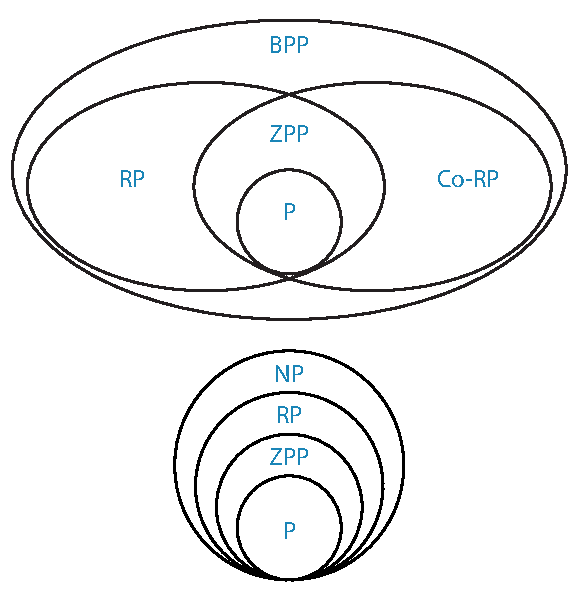
\includegraphics[width=.8\textwidth]{Graphics/Relationships}
	\caption{Beziehungen zwischen den Komplexitätsklassen}
	\label{fig:cc_relationships}
\end{figure}
\paragraph{Beobachtung}
Auf den ersten Blick ähneln sich P und ZPP sehr.
Es gilt aber zu beachten, dass für die Sprachen in ZPP lediglich die erwartete Ausführungszeit polynomiell sein muss, während die WCET auch deutlich schlechter sein kann.

\paragraph{Aufgabe}
Welche Beziehung besteht zwischen P und ZPP?

\paragraph{Satz}
$P \subseteq ZPP$

\paragraph{Beweis}
Jede polynomielle deterministische Turingmaschine ist ebenfalls eine polynomielle Las-Vegas-Turinmaschine, die aber ihre Fähigkeit nicht nutzt, eine zufällige Auswahl zu treffen.

\paragraph{Satz}
$RP \subseteq NP$

\paragraph{Beweis}
Wir nehmen an, es gibt eine Monte-Carlo-Turingmaschine $M_1$, $L(M_1) = L$.
Wir können eine äquivalente, nichtdeterministische Turingmaschine $M_2$ mit gleicher Zeitbegrenzung konstruieren:
\begin{itemize}
	\item $M_2$ \emph{rät} stets das Zufallsbit von $M_1$ und legt es auf ein Hilfsband.
	\item \begin{equation*}
		M_2 =
		\begin{cases}
			akzeptiert &,\ M_1\ akzeptiert\\
			akzeptiert\ nicht &,\ sonst
		\end{cases}
	\end{equation*}
\end{itemize}
Folgerung:
\begin{align*}
	w \in &\Rightarrow \text{Es gibt eine erfolgreiche Berechnung, die }M_2\text{ raten kann}\\
	w \notin &\Rightarrow \text{Es gibt keine erfolgreiche Berechnung, die }M_2\text{ raten kann}
\end{align*}